\section{Experimental Evaluation}
\label{sec:experiment}

In this section, we conduct a practical evaluation through experimentation in which we instantiate the semantic models aforementioned for a real scientific workflow application. We study and document the Montage~\cite{Montage} workflow and its execution environment, which includes the application software components and the workflow management system. Montage is an astronomy workflow application that is widely used by many astronomers to construct large image mosaics of the sky.

The goal of this experiment is to reproduce original workflow executions in two different 
Cloud infrastructures: FutureGrid~\cite{futuregrid} and Amazon EC2~\cite{aws}. 
FutureGrid is an academic Cloud test-bed facility that includes a number of computational 
resources at distributed locations. Amazon Web Services EC2 is a public infrastructure 
provider and the \emph{de facto} standard for IaaS Cloud platforms.


\subsection{Scientific Workflows}

\paragraph{\textbf{Montage}}
The Montage workflow~\cite{Montage} was created by the NASA Infrared Processing 
and Analysis Center (IPAC) as an open source toolkit that can be used to generate 
custom mosaics of astronomical images in the Flexible Image Transport System (FITS) 
format. In a Montage workflow, the geometry of the output mosaic is calculated from the 
input images. The inputs are then re-projected to have the same spatial scale and rotation, 
the background emissions in the images are corrected to have a uniform level, and the 
re-projected, corrected images are co-added to form the output mosaic. 
Figure~\ref{fig:workflow-montage} illustrates a small (20 node) Montage workflow. The 
size of the workflow depends on the number of images required to construct the desired 
mosaic. The workflow instance used in this paper generate a 0.1 degree square mosaics 
using 15 input images from the 2 Micron All Sky Survey (2MASS).

\begin{figure}[!htt]
	\centering
	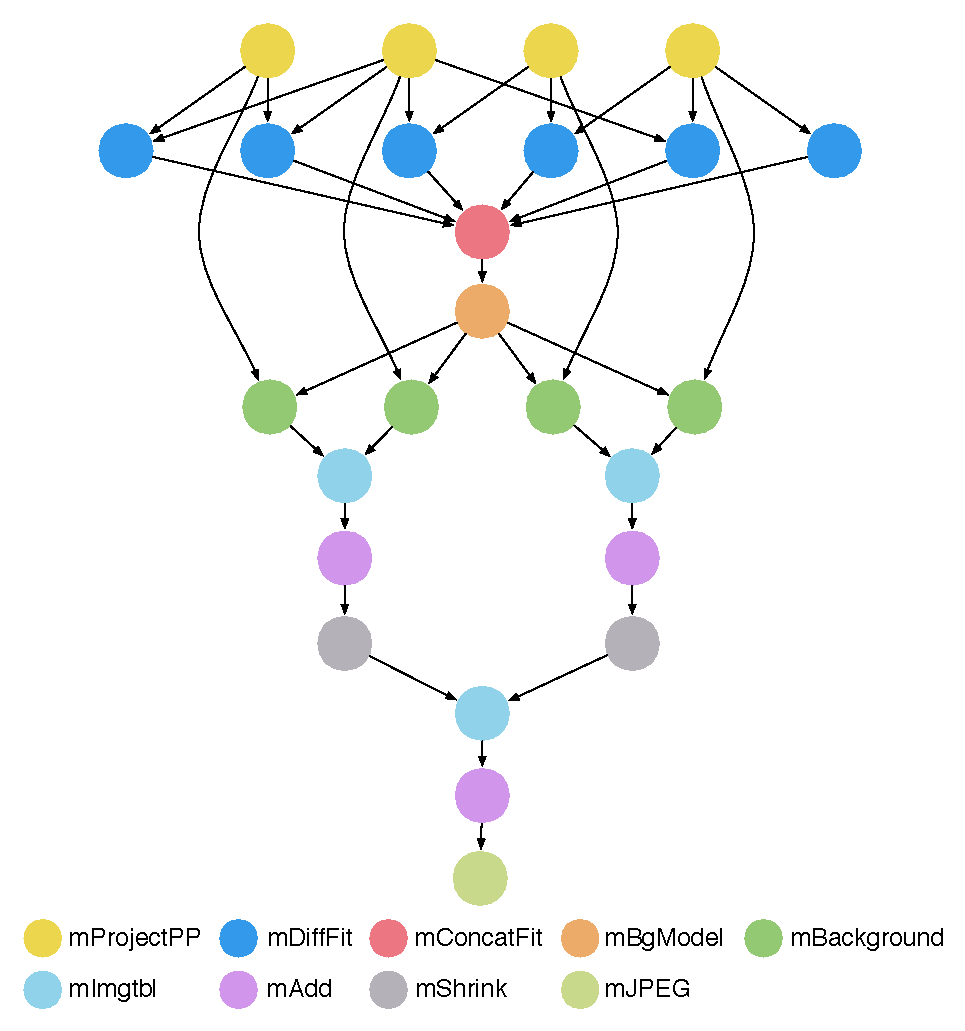
\includegraphics[width=0.9\linewidth]{figures/workflow-montage}
	\caption{A small (20 node) Montage workflow.}
	\label{fig:workflow-montage}
\end{figure}


\paragraph{\textbf{Epigenomics}}
The USC Epigenome Center~\cite{genome} is currently involved in mapping the epigenetic 
state of human cells on a genome-wide scale. The Epigenomics workflow 
(Figure~\ref{fig:workflow-genome}) processes multiple sets of genome sequences in
parallel. These sequences are split into subsets, the subsets are filtered to remove
contaminants, reformatted, then mapped to a reference genome. The mapped sequences are
finally merged and indexed for later analysis. In this work, the Epigenome workflow was 
used to align 13 million genome sequence reads to a reference genome for human 
chromosome 21. The size of the workflow depends on the chunking factor used on the input 
data (\texttt{binsize}), which determines the number of sequence reads in each chunk.

\begin{figure}[!htb]
	\centering
	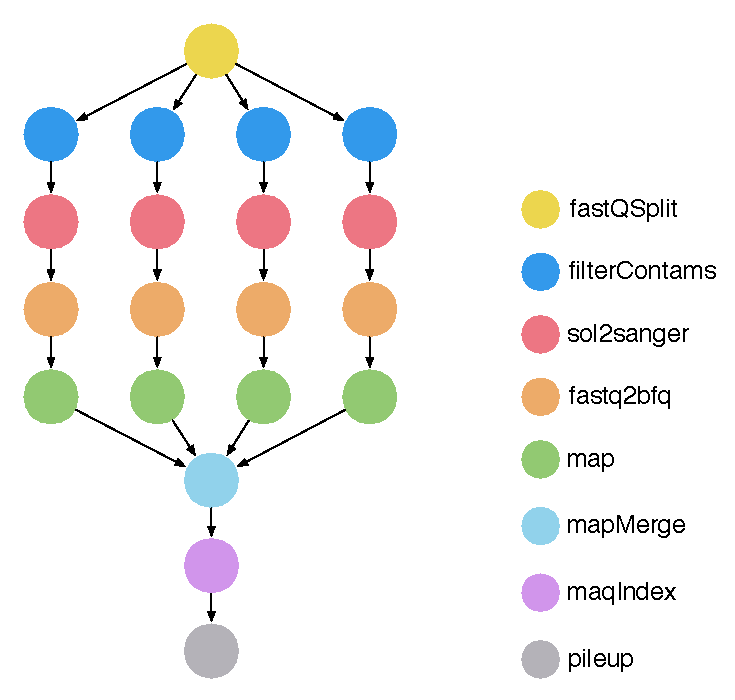
\includegraphics[width=0.75\linewidth]{figures/workflow-genome}
	\caption{Epigenomics workflow.}
	\label{fig:workflow-genome}
\end{figure}

\paragraph{\textbf{SoyKB}}
The SoyKB workflow~\cite{soybean, Joshi01012014} is a genomics pipeline 
that re-sequences soybean germplasm lines selected for desirable traits such 
as oil, protein, soybean cyst nematode resistance, stress resistance, and root 
system architecture. The workflow (Figure~\ref{fig:workflow-soykb}) 
implements a SNP and injection/deletion (indel) identification and analysis 
pipeline using the GATK haplotype caller~\cite{gatk} and a soybean reference 
genome. The workflow analyzes samples in parallel to align them to the reference 
genome, to de-duplicate the data, to identify indels and SNPs, and to merge and 
filter the results. The results are then used for genome-wide association studies 
(GWAS) and genotype to phenotype analysis. The workflow instance used in this 
paper is based on a sample dataset of 50 sequence reads that requires less 
memory than a full-scale production workflow.

\begin{figure}[!htb]
	\centering
	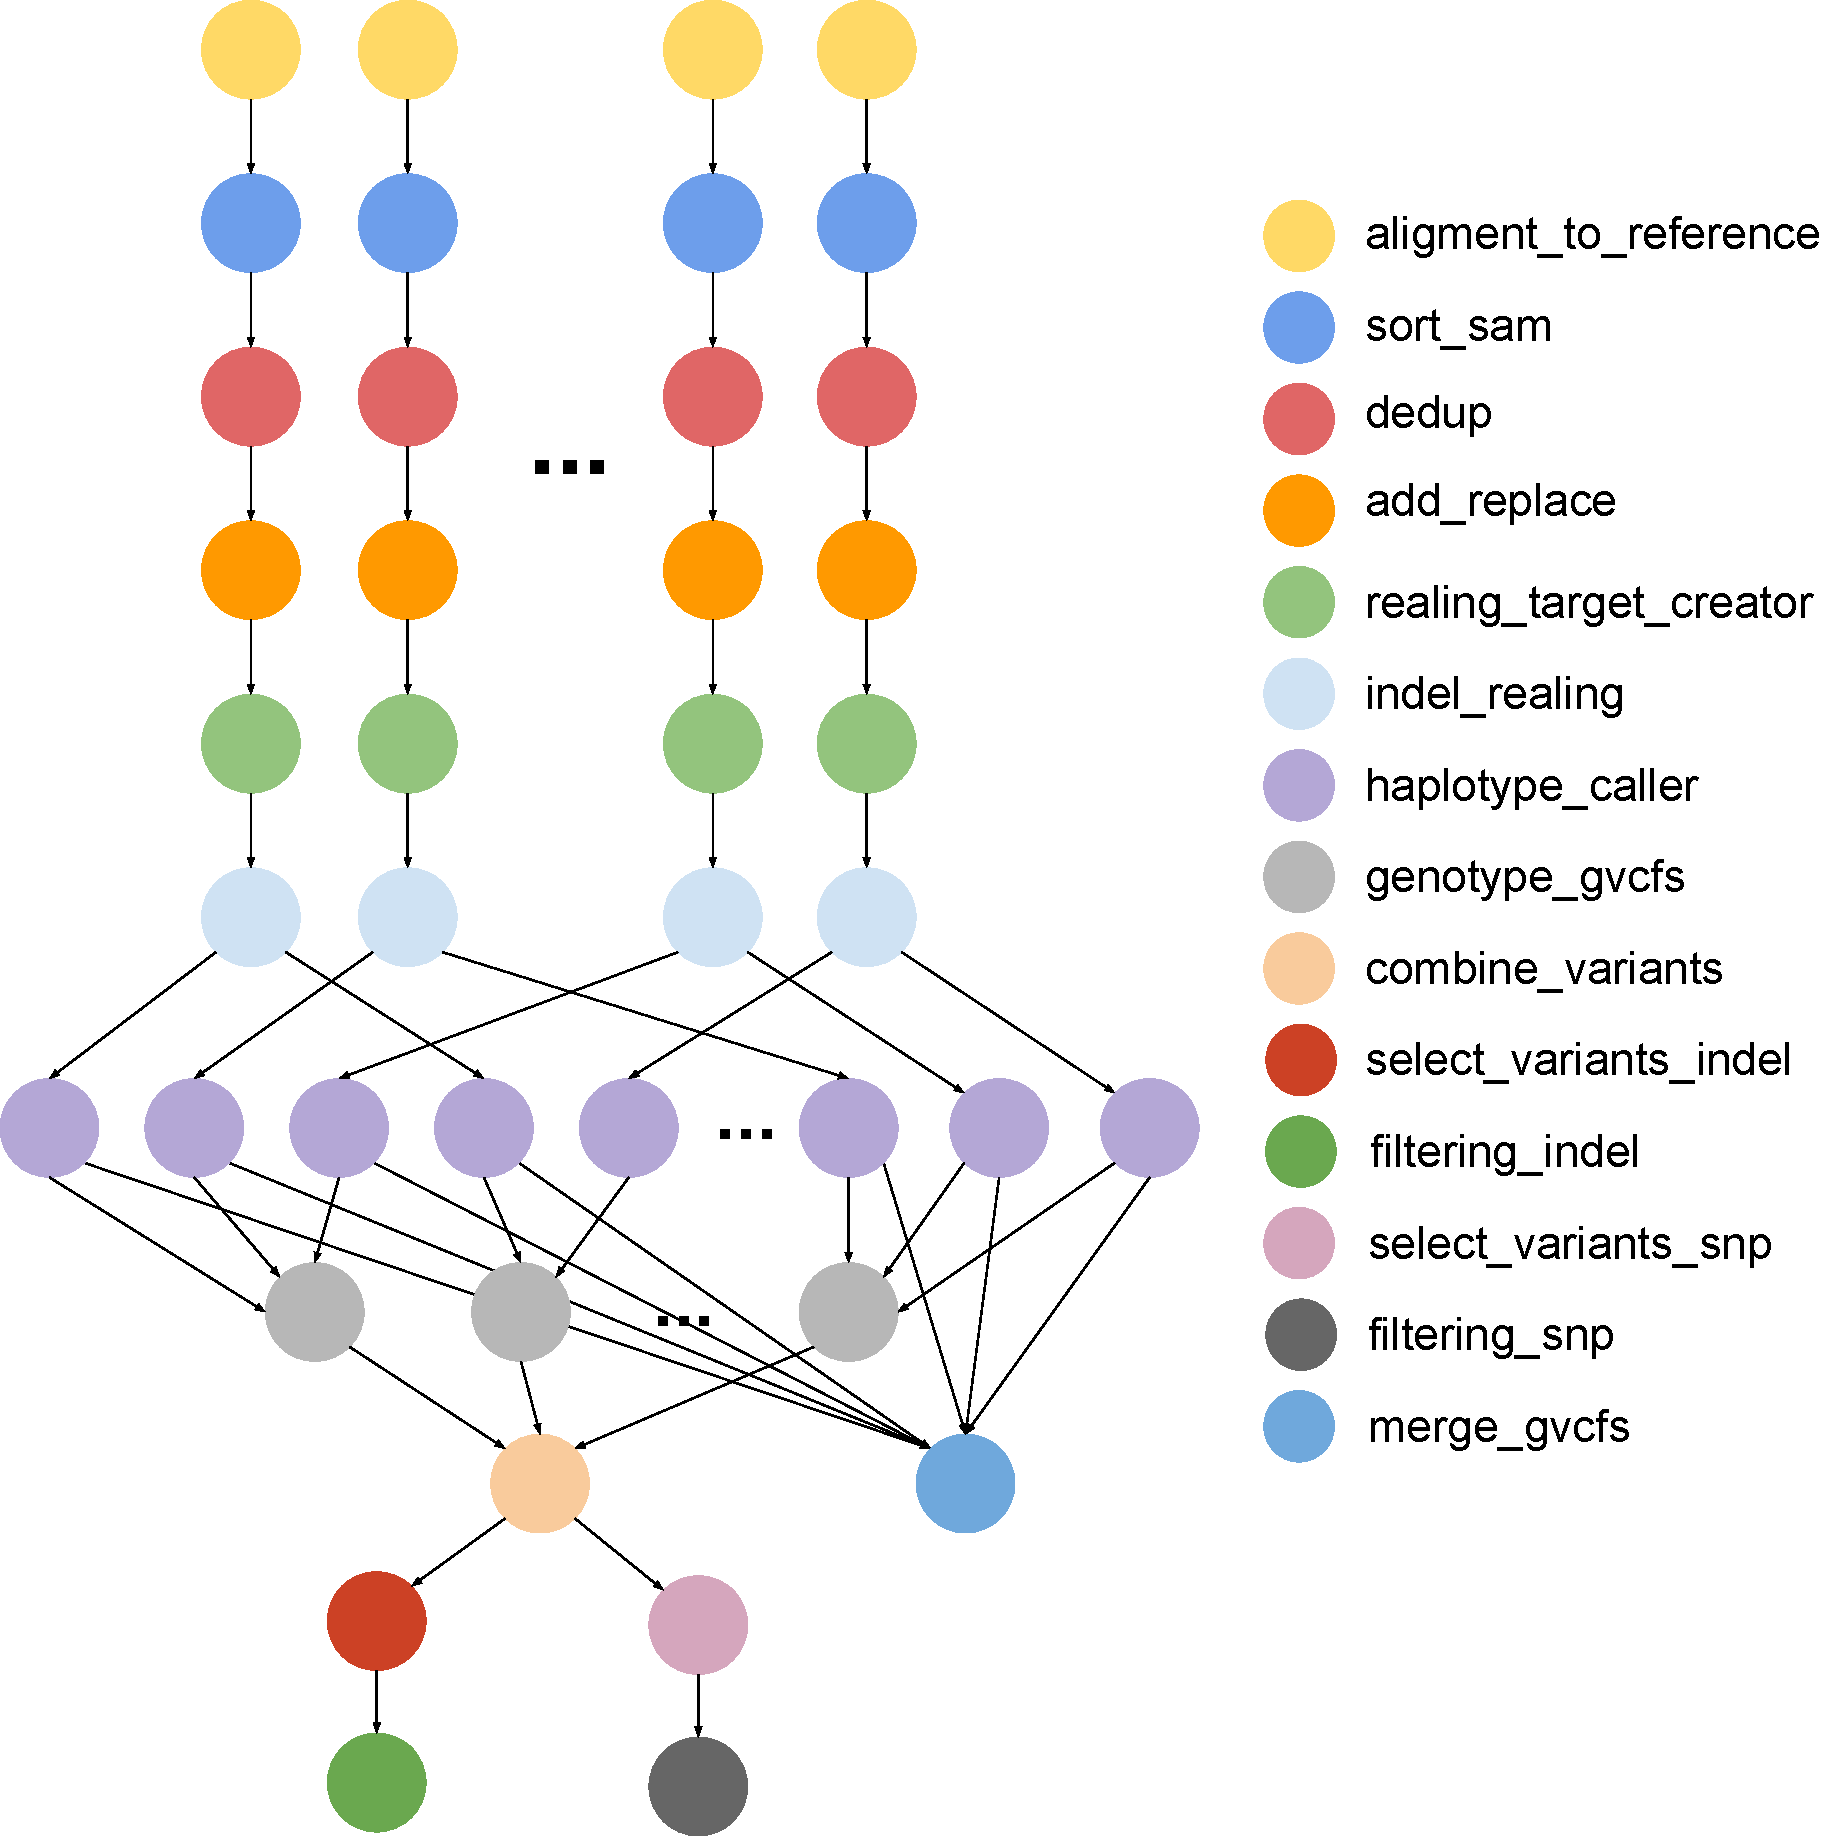
\includegraphics[width=0.95\linewidth]{figures/workflow-soybean}
	\caption{SoyKB workflow.}
	\label{fig:workflow-soykb}
\end{figure}


% Generating Semantic Annotations
\subsection{Generating Semantic Annotations}

\paragraph{\textbf{Montage}}
Figure~\ref{fig:annotations} shows a simplified overview of the annotations generated for the Montage workflow using the WICUS ontology network.

\begin{figure}[!htb]
	\centering
	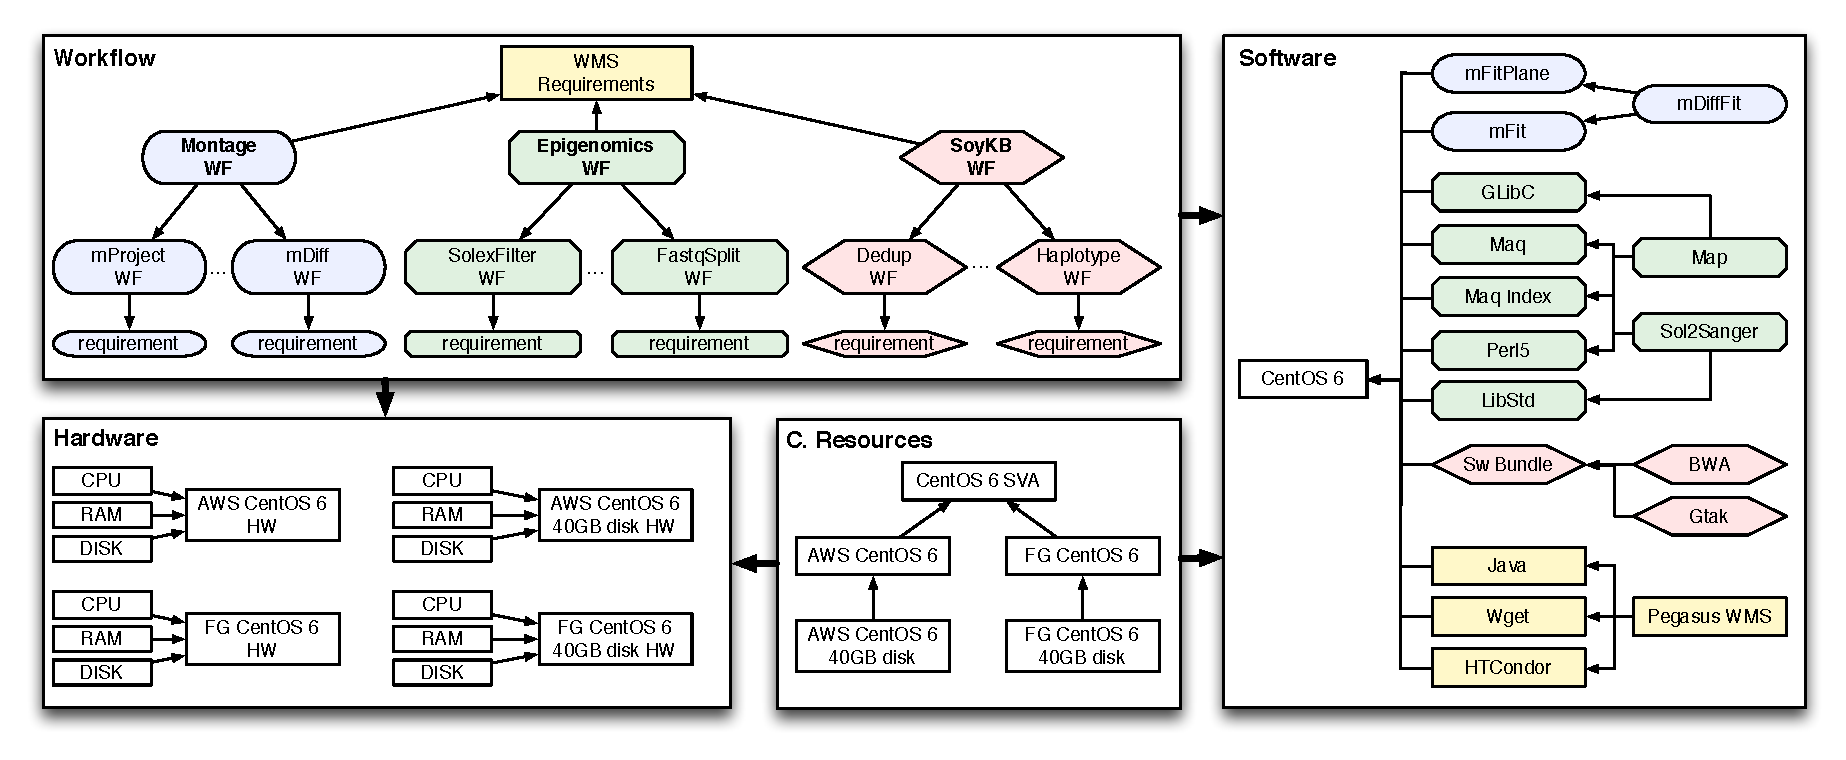
\includegraphics[width=\linewidth]{figures/annotations}
	\caption{Annotations for the Montage workflow using the WICUS ontology network.}
	\label{fig:annotations}
\end{figure}

As shown in Figure~\ref{fig:wicusflow}, the first step in the process of documenting a workflow is the annotation of the workflow DAX file. We use the \texttt{Workflow} domain ontology to describe the Montage workflow as 1) an individual that represents the top level workflow, and 2) another 9 individuals representing its sub-workflows, one for each transformation. We also generate 10 requirements, one for the top level workflow, which specifies the WMS requirements, and the remaining for defining the software components required by each transformation. At this point, these requirements are empty, as they are not yet related to their software components.
 
In this experiment, we address two types of components: the WMS and the application related components. The WMS components include the workflow engine, in our case the Pegasus WMS, and its dependencies. Pegasus uses HTCondor as task manager, and also depends on Java. We use the \texttt{Software} domain ontology to describe these components as individuals, and to represent their dependencies. The 3 components also depend on the operating system, which in our case is CentOS.

To describe the deployment of the WMS components, we studied their installation processes according to their documentation. We then defined a set of installation bash scripts for each of them. These scripts are included on the deployment plans of the components along with their configuration information.  
 
Application components are described from the Montage workflow's Transformation Catalog, where the binary file, version, and destination path are defined. These components are also described as individuals using the \texttt{Software} domain ontology. We use this information to generate the configuration parameters of the deployment script, which in this case is the same for all components. The script downloads the binary files from an online repository and copies them to the specified destination path. This process identified 59 software components for the Montage workflow that are annotated and included in the Software Components Catalog.
Then, the Transformation Catalog Annotator module relates each transformation requirement, defined using the \texttt{Workflow} domain ontology, to the application component, and therefore to the deployment information.
In this experiment, we define 9 Montage components that are linked to the requirements, and another two sub-components that are defined as dependencies in the software catalog (\emph{mDiffFit} depends on the \emph{mDiff} and \emph{mFitPlane} components).

To describe computational resources we use the \texttt{Computing Resources} and \texttt{Hardware} domain ontologies. The Scientific Virtual Appliances Catalog includes the description of two virtual machine images, one for FutureGrid and another for Amazon EC2. These two images are conceptually equivalent, as they both provide CentOS 6 operating system.
Therefore, we generate two Image Appliances (FG CentOS 6 and AWS CentOS 6) that are grouped into one single Scientific Virtual Appliance (CentOS 6 SVA). Depending on which providers are available, one or the other will be selected.


\subsection{Reproducing Workflow Executions.}

The last step on the process for achieving reproducibility in scientific workflows (Figure~\ref{fig:wicusflow}) is to execute the Infrastructure Specification Algorithm (ISA). The ISA combines the annotated data based on the 4 domain ontologies in order to find a suitable infrastructure specification that is able to run the workflow. The algorithm retrieves and propagates the WMS requirements of the top-level workflow (\texttt{Workflow} domain ontology) to its related sub-workflows. Requirements and software components are matched, and a dependency graph is built based on the relation between the requirements and the component dependencies. This graph is then used to compute the intersection between the set of software components from the SVA and the dependency graph of each sub-workflow. ISA selects the intersection where the value is maximized for each sub-workflow. Software components already available in the SVA are then removed from the chosen graph. To reduce the number of SVAs, the algorithm attempts to merge sub-workflows requirements into a single SVA. Requirements can be merged if all their software components are compatible. Finally, ISA generates a PRECIP script with the set of required instructions to instantiate, configure, and deploy the computational resources and software components.


In this experiment, we execute ISA over the annotated data in a scenario where FutureGrid is the only available platform for resource provisioning, and in a scenario where the available platform is Amazon EC2. In both cases, the algorithm is able to obtain a PRECIP script for each infrastructure. Each generated script is composed by the following main sections:

\begin{itemize}

	\item \emph{Experiment Creation}: generates a new experiment using the given VM image ID and the user credentials for the selected infrastructure provider;
    	    
	\item \emph{Software Deployment}: executes the set of instructions defined on the deployment plan of each software component to install and configure the required software to execute the workflow. In this section, both the workflow management system and the application are deployed with their dependencies;

	\item \emph{User Setup}: creates a user account on the VM (if it does not exist) and configures the necessary SSH keys to enable file transfers and execution. This account will be used to run the workflow;
	   
	\item \emph{Data Stage and Workflow Execution}: stages all the input data of the Montage workflow on the VM, and launches the workflow execution. Since our work is focused on infrastructure reproducibility, data and workflow management are not covered in our approach.

\end{itemize}

\noindent Note that all the configuration and deployment commands (first 3 sections) require superuser privileges on the VM. The workflow execution, however, is performed under the user account created in the third section.

We executed the scripts on their corresponding platforms. Both executions succeeded on deploying and running the Montage workflow, the Pegasus WMS, and their dependencies. We also performed the same execution of the Montage workflow in a predefined VM image, where the execution environment is already in place. Results show that the VM execution environments deployed by both scripts are equivalent to the former one. In addition, we used a perceptual hash tool\footnote{pHash - \url{http://www.phash.org}} to compare the resulting image (0.1 degree image of the sky) generated by both executions against the one generated by the baseline execution. We obtained a similarity factor of 1.0 (over 1.0) with a threshold of 0.85, which means the images are identical. Therefore we are obtaining the same results as the original workflow. In this work we do not aim to reproduce either the performance or the execution time of the original experiment.


All the original and generated scripts are available as part of the experimental material included in the Research Object (RO)~\cite{researchObjects} associated with this paper\footnote{\url{http://pegasus.isi.edu/publications/reppar}}. This RO also contains pointers to the software and resources used in this experiment.